\PassOptionsToPackage{unicode}{hyperref}
\PassOptionsToPackage{naturalnames}{hyperref}

\documentclass[10pt]{beamer}

\usetheme[sectionpage=none,block=fill]{metropolis}

\usepackage{acronym} % \ac[p], \acl[ptl], \acs[p], \acf[p]
\usepackage{algorithm, algpseudocode}
\usepackage{appendixnumberbeamer}
\usepackage[backend=biber,style=alphabetic,sorting=none,maxbibnames=1]{biblatex}
\usepackage{amsmath, amssymb, amsthm}
\usepackage{bookmark}
\usepackage{booktabs} % \toprule, \midrule, \cmidrule, \bottomrule
\usepackage{cancel} % \cancel
\usepackage{caption}
\usepackage[scale=2]{ccicons}
\usepackage{csquotes} % Dépendance de babel
\usepackage{graphicx}
\hypersetup{hidelinks}
% \usepackage[inline]{enumitem}
% \setlist[enumerate]{label=(\roman*)} %% <- set the base level label separately
\usepackage{marvosym} % \Flatsteel
\usepackage{MnSymbol} % \dashrightarrow
\usepackage{pifont} % \ding
\usepackage{silence} % \WarningFilter
\WarningFilter{biblatex}{Patching footnotes failed}
\usepackage{subcaption} % subfigure
\usepackage{tikz} % \begin{tikzpicture} \end{tikzpicture}
\usetikzlibrary{calc}
\usetikzlibrary{graphs}
\usetikzlibrary{positioning}
\usetikzlibrary{quotes}
\usetikzlibrary{shapes.misc}
\usetikzlibrary{tikzmark}
\usepackage{wasysym} % \checked
\usepackage{xcolor}
\usepackage{xspace} % \xspace

%-------------------------------------------------------------------
%                           Assets
%-------------------------------------------------------------------
\acrodef{ADT}[ADT]{Abstract Data Type}
\acrodefplural{ADT}[ADTs]{Abstract Data Types}
\acrodef{API}[API]{Application Programming Interface}
\acrodef{AW}[AW]{Add-Wins}
\acrodef{CCI}[CCI]{Convergence, Causality preservation, Intention preservation}
\acrodef{CL}[CL]{Causal-Length}
\acrodef{CRDT}[CRDT]{Conflict-free Replicated Data Type}
\acrodefplural{CRDT}[CRDTs]{Conflict-free Replicated Data Types}
\acrodef{DAG}[DAG]{Directed Acyclic Graph}
\acrodef{FIFO}[FIFO]{First In, First Out}
\acrodef{GC}[GC]{Garbage Collection}
\acrodef{IPFS}[IPFS]{InterPlanetary File System}
\acrodef{JIT}[JIT]{Just-In-Time}
\acrodef{LCA}[PPAC]{Plus Petit Ancêtre Commun}
\acrodef{LFS}[LFS]{Local-First Software}
\acrodef{LUB}[LUB]{Least Upper Bound}
\acrodef{LWW}[LWW]{Last-Writer-Wins}
\acrodef{MUTE}[MUTE]{Multi User Text Editor}
\acrodef{MV}[MV]{Multi-Value}
\acrodef{OC}[OC]{Commutativité des Opérations}
\acrodef{OT}[OT]{Operational Transformation}
\acrodefplural{OT}[OT]{Operational Transformations}
\acrodef{P2P}[P2P]{pair-à-pair}
\acrodef{PKI}[PKI]{Public Key Infrastructure}
\acrodef{PoC}[PoC]{Proof of Concept}
\acrodef{PT}[PT]{Transitivité de la Précédence}
\acrodef{RADT}[RADT]{Replicated Abstract Data Type}
\acrodefplural{RADT}[RADTs]{Replicated Abstract Data Types}
\acrodef{RCB}[RCB]{Reliable Causal Broadcast}
\acrodef{RGA}[RGA]{Replicated Growable Array}
\acrodef{RW}[RW]{Remove-Wins}
\acrodef{SEC}[SEC]{Cohérence forte à terme}
\acrodef{SPOF}[SPOF]{Single Point Of Failure}
\acrodef{TTF}[TTF]{Tombstone Transformation Function}
\acrodefplural{TTF}[TTF]{Tombstone Transformation Functions}
\acrodef{WebRTC}[WebRTC]{Web Real-Time Communication}

\floatname{algorithm}{Algorithme} % Renomme caption de "Algorithm" -> "Algorithme"

\newcommand\CONDITION[2]%
  {\begin{tabular}[t]{@{}l@{}l@{}}
     #1&#2
   \end{tabular}%
  }
  \algdef{SE}[WHILE]{While}{EndWhile}[1]%
  {\algorithmicwhile\ \CONDITION{#1}{\ \algorithmicdo}}%
  {\algorithmicend\ \algorithmicwhile}
\algdef{SE}[FOR]{For}{EndFor}[1]%
  {\algorithmicfor\ \CONDITION{#1}{\ \algorithmicdo}}%
  {\algorithmicend\ \algorithmicfor}
\algdef{S}[FOR]{ForAll}[1]%
  {\algorithmicforall\ \CONDITION{#1}{\ \algorithmicdo}}
\algdef{SE}[REPEAT]{Repeat}{Until}{\algorithmicrepeat}[1]%
  {\algorithmicuntil\ \CONDITION{#1}{}}
\algdef{SE}[IF]{If}{EndIf}[1]%
  {\algorithmicif\ \CONDITION{#1}{\ \algorithmicthen}}%
  {\algorithmicend\ \algorithmicif}%
\algdef{C}[IF]{IF}{ElsIf}[1]%
  {\algorithmicelse\ \algorithmicif\ \CONDITION{#1}{\ \algorithmicthen}}

\newcommand{\commentbott}{with $\bott$ the minimal tuple}
\newcommand{\commenttopt}{with $\topt$ the maximal tuple}

\newcommand{\algorithmautorefname}{Algorithme}
\newcommand{\annexautorefname}{Annexe}
\newcommand{\definitionautorefname}{Définition}
\newcommand{\propertyautorefname}{Propriété}
% \newcommand{\subfigureautorefname}{Figure}
\newcommand{\subpropertyautorefname}{Propriété}

\addbibresource{biblio.bib}
\AtBeginBibliography{\footnotesize}
% \setbeamertemplate{bibliography item}[text] % use ref number in bibliography

\renewcommand{\thefootnote}{[\arabic{footnote}]}
    % Footnote style: [footnote-counter]

\newcommand\singlefootnote[1]{%
    % Use this footnote variant when a single footnote is on the page
    % Footnote style: *
    \begingroup
    %\renewcommand\thefootnote{}\footnote{#1}%
    \renewcommand{\thefootnote}{*}\footnote{#1}%
    \addtocounter{footnote}{-1}%
    \endgroup
}

\AtBeginDocument{
\definecolor{lfsgreen}{RGB}{31,160,31}
\definecolor{lfsorange}{RGB}{255,178,2}
\definecolor{lfsred}{RGB}{160,30,31}

% white
\definecolor{uclwhite}{rgb}{1, 1, 1}

%   UCL style guide colours.
%   Number refer to level of tint.
%   100%    1
%    70%    2
%    50%    3
%    20%    4

 % UCL style guide dk purple
\definecolor{ucl1dkpurple}{RGB}{82,66,91}
\definecolor{ucl2dkpurple}{RGB}{134,122,140}
\definecolor{ucl3dkpurple}{RGB}{168,160,173}
\definecolor{ucl4dkpurple}{RGB}{220,217,222}

 % UCL style guide dk red
\definecolor{ucl1dkred}{RGB}{90,27,49}
\definecolor{ucl2dkred}{RGB}{139,95,110}
\definecolor{ucl3dkred}{RGB}{172,141,152}
\definecolor{ucl4dkred}{RGB}{222,209,214}

 % UCL style guide dk blue
\definecolor{ucl1dkblue}{RGB}{0,67,89}
\definecolor{ucl2dkblue}{RGB}{76,123,138}
\definecolor{ucl3dkblue}{RGB}{127,161,172}
\definecolor{ucl4dkblue}{RGB}{204,217,222}

 % UCL style guide dk green
\definecolor{ucl1dkgreen}{RGB}{75,70,32}
\definecolor{ucl2dkgreen}{RGB}{129,125,98}
\definecolor{ucl3dkgreen}{RGB}{165,162,143}
\definecolor{ucl4dkgreen}{RGB}{219,218,210}

 % UCL style guide black
\definecolor{ucl1black}{RGB}{0,0,0}
\definecolor{ucl2black}{RGB}{75,75,75}
\definecolor{ucl3black}{RGB}{128,128,128}
\definecolor{ucl4black}{RGB}{205,205,205}

 % UCL style guide pink
\definecolor{ucl1pink}{RGB}{145,24,83}
\definecolor{ucl2pink}{RGB}{178,93,134}
\definecolor{ucl3pink}{RGB}{200,139,169}
\definecolor{ucl4pink}{RGB}{233,209,221}

 % UCL style guide md red
\definecolor{ucl1mdred}{RGB}{195,58,45}
\definecolor{ucl2mdred}{RGB}{213,117,108}
\definecolor{ucl3mdred}{RGB}{225,156,150}
\definecolor{ucl4mdred}{RGB}{243,216,213}

 % UCL style guide md blue
\definecolor{ucl1mdblue}{RGB}{69,156,189}
\definecolor{ucl2mdblue}{RGB}{124,186,209}
\definecolor{ucl3mdblue}{RGB}{162,205,222}
\definecolor{ucl4mdblue}{RGB}{218,235,242}

 % UCL style guide md green
\definecolor{ucl1mdgreen}{RGB}{130,141,55}
\definecolor{ucl2mdgreen}{RGB}{167,175,115}
\definecolor{ucl3mdgreen}{RGB}{192,198,155}
\definecolor{ucl4mdgreen}{RGB}{230,232,215}

 % UCL style guide orange
\definecolor{ucl1orange}{RGB}{215,123,35}
\definecolor{ucl2orange}{RGB}{227,162,101}
\definecolor{ucl3orange}{RGB}{235,189,145}
\definecolor{ucl4orange}{RGB}{247,229,211}

  % UCL style guide lt purple
\definecolor{ucl1ltpurple}{RGB}{191,175,188}
\definecolor{ucl2ltpurple}{RGB}{210,199,208}
\definecolor{ucl3ltpurple}{RGB}{223,215,221}
\definecolor{ucl4ltpurple}{RGB}{242,239,242}

 % UCL style guide yellow
\definecolor{ucl1yellow}{RGB}{229,175,0}
\definecolor{ucl2yellow}{RGB}{237,199,76}
\definecolor{ucl3yellow}{RGB}{242,215,127}
\definecolor{ucl4yellow}{RGB}{250,239,204}

 % UCL style guide lt blue
\definecolor{ucl1ltblue}{RGB}{168,192,209}
\definecolor{ucl2ltblue}{RGB}{194,211,223}
\definecolor{ucl3ltblue}{RGB}{211,223,232}
\definecolor{ucl4ltblue}{RGB}{238,242,246}

% UCL style guide brt green
\definecolor{ucl1brtgreen}{RGB}{204,209,88}
\definecolor{ucl2brtgreen}{RGB}{219,223,138}
\definecolor{ucl3brtgreen}{RGB}{229,232,171}
\definecolor{ucl4brtgreen}{RGB}{245,246,222}

% UCL style guide stone
\definecolor{ucl1stone}{RGB}{217,214,204}
\definecolor{ucl2stone}{RGB}{228,226,219}
\definecolor{ucl3stone}{RGB}{236,234,229}
\definecolor{ucl4stone}{RGB}{255,255,255}

% UCL style guide lt green
\definecolor{ucl1ltgreen}{RGB}{185,193,147}
\definecolor{ucl2ltgreen}{RGB}{206,211,179}
\definecolor{ucl3ltgreen}{RGB}{220,224,201}
\definecolor{ucl4ltgreen}{RGB}{241,243,233}

\definecolor{darkgreen}{RGB}{75,70,32}
\definecolor{darkblue}{RGB}{0,67,89}
}

\newcommand{\colorblockone}{ucl2orange}
\newcommand{\coloridone}{\color{ucl1orange}}

\newcommand{\colorblocktwo}{ucl2mdblue}
\newcommand{\coloridtwo}{\color{ucl2dkblue}}

\newcommand{\colorblockthree}{ucl3orange}
\newcommand{\coloridthree}{\color{ucl1orange}}

\newcommand{\colorblockfour}{ucl3mdblue}
\newcommand{\coloridfour}{\color{ucl2dkblue}}

\newcommand{\colorblockfive}{ucl1ltpurple}
\newcommand{\coloridfive}{\color{ucl2dkpurple}}

\newcommand{\colorcross}{ucl1mdred}
\newcommand{\colorcurrentepoch}{ucl1mdblue}
\newcommand{\colortargetepoch}{ucl1mdred}


\newcommand{\widthletter}{2em}
\newcommand{\widthblock}{3em}
\newcommand{\widthoriginepoch}{1.33em}
\newcommand{\widthepoch}{1.65em}

\newcommand{\bott}{\bot_t}
\newcommand{\epoch}[1]{\varepsilon_{#1}}
\newcommand{\id}[3]{\trm{#1}^{\trm{#2}}_{\trm{#3}}}
\newcommand{\lepoch}{<_{\varepsilon}}
\newcommand{\lid}{<_{id}}
\newcommand{\logootsplituple}[1]{\langle \text{pos}_{#1},\text{nodeId}_{#1},\text{nodeSeq}_{#1},\text{offset}_{#1} \rangle}
\newcommand{\logootuple}[1]{\langle \text{pos}_{#1},\text{nodeId}_{#1},\text{nodeSeq}_{#1} \rangle}
\newcommand{\lstatus}{<_{s}}
\newcommand{\ltuple}{<_{t}}
\newcommand{\ltupleupdated}{<_{t'}}
\newcommand{\newFirstId}{\langle \text{pos},\text{nodeId},\text{nodeSeq},0 \rangle}
\newcommand{\newLastId}{\langle \text{pos},\text{nodeId},\text{nodeSeq},n-1 \rangle}
\newcommand{\newlogootsplituple}[1]{\langle \text{pos},\text{nodeId},\text{nodeSeq},{#1} \rangle}
\newcommand{\predNewFirstId}{\langle \text{pos},\text{nodeId},\text{nodeSeq},-1 \rangle}
\newcommand{\renids}[1]{\trm{renIds}_{#1}}
\newcommand{\topt}{\top_t}

% \interdisplaylinepenalty=2500
\theoremstyle{definition}
% \newtheorem{definition}{Définition}
% \newtheorem{subdefinition}{Définition}[definition]
\newtheorem{myrule}{Règle}
\newtheorem{property}{Propriété}
\newtheorem{subproperty}{Propriété}[property]

\newcommand{\bigO}[1]{$\mathcal{O}(#1)$}
\newcommand{\botn}{\bot_\nat}
\newcommand{\topn}{\top_\nat}
\newcommand{\elt}{E}
\newcommand{\inbb}[1]{\in \mathbb{#1}}
\newcommand{\nat}{\mathbb{N}}
\newcommand{\set}[1]{\left\{#1\right\}} % set brace notation
\newcommand{\trm}[1]{\mathit{#1}}
\newcommand{\withmathbreak}[1]{\parbox{\linewidth}{#1}}

\newcommand{\cf}[1]{(cf. \autoref{#1}, page \pageref{#1})}
\newcommand{\eg}{e.g.\xspace}
\newcommand{\ie}{c.-à-d.\xspace}

\renewcommand{\checkmark}{\ding{51}}
\newcommand{\ballotx}{\ding{55}}

\newcommand{\hb}{\emph{happens-before}\xspace}

\newcommand{\new}{\textbf{new}}

\newcommand{\ins}{\emph{insert}\xspace}
\newcommand{\ren}{\emph{rename}\xspace}
\newcommand{\rmv}{\emph{remove}\xspace}

\tikzset{
    common/.style={anchor=west, draw, rectangle, minimum height=6mm},
    letter/.style={common, minimum width=\widthletter},
    block/.style={common, minimum width=\widthblock},
    epoch/.style={letter, rounded rectangle, rounded rectangle east arc=0pt, minimum width=\widthepoch},
    point/.style={insert path={ node[scale=5*sqrt(\pgflinewidth)]{.} }},
    node/.style={draw, circle, minimum size=1em},
    op/.style={draw, circle, minimum size=2.7em},
    causalop/.style={op, double=white, inner sep=2pt},
    gc-rule-1/.style={dashed, thick, darkblue},
    gc-rule-2/.style={densely dotted, thick, darkgreen},
    cross/.style={
        path picture={
            \draw[\colorcross, very thick]
                (path picture bounding box.south east)--(path picture bounding box.north west)
                (path picture bounding box.south west)--(path picture bounding box.north east);
        }
    },
    currentepoch/.style={\colorcurrentepoch},
    targetepoch/.style={\colortargetepoch},
    invisible/.style={opacity=0},
    visible on/.style={alt=#1{}{invisible}},
    alt/.code args={<#1>#2#3}{%
      \alt<#1>{\pgfkeysalso{#2}}{\pgfkeysalso{#3}} % \pgfkeysalso doesn't change the path
    },
}


\author{
  \textbf{Matthieu Nicolas} (\texttt{matthieu.nicolas@inria.fr})
}
\date{02/05/2024}
\title{Conflict-free Replicated Data Types (CRDTs)}
\subtitle{An Overview}
%\institute{}

\begin{document}

\begin{frame}[t,plain]
  \maketitle
\end{frame}

\section{Data replication in peer-to-peer systems}

\begin{frame}{MUTE \cite{MUTE2017}}
    \vspace{-0.5cm}
    \begin{figure}
        \resizebox{\textwidth}{!}{
            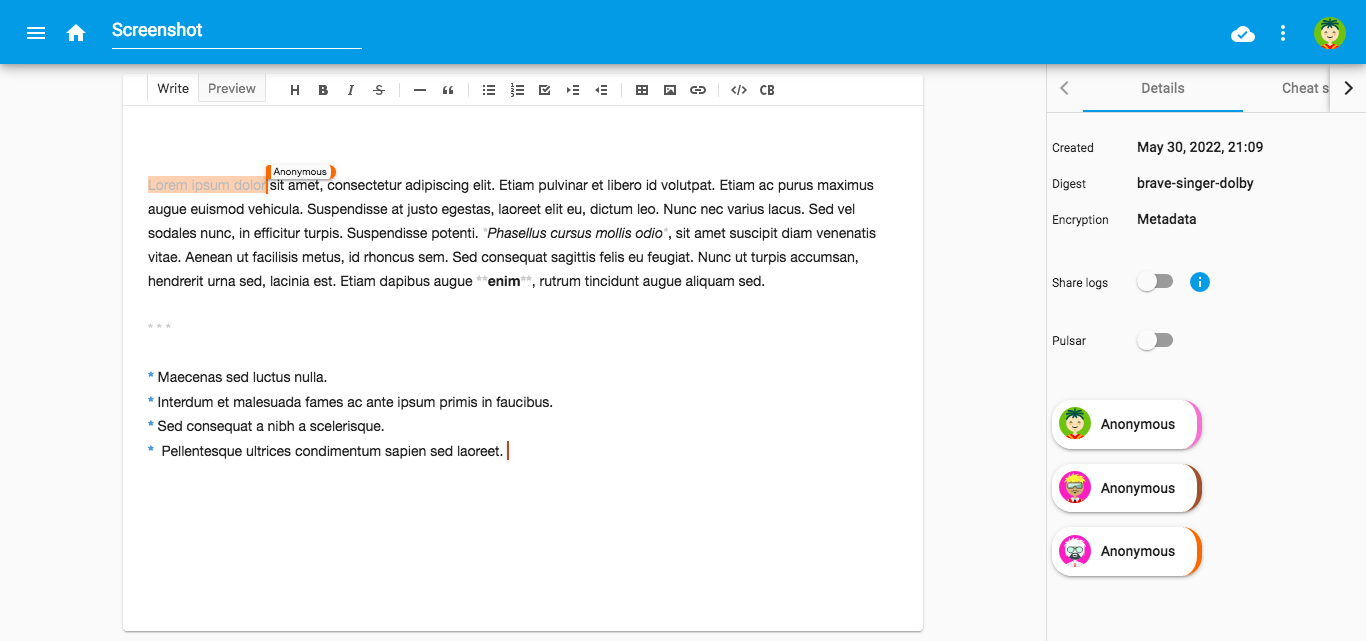
\includegraphics{img/screenshot-mute-editor.png}
        }
    \end{figure}
    \vspace{-0.5cm}
    \begin{itemize}
        \item Peer-to-Peer (P2P) application \cite{localfirstsoftware2019}
        \item Allow to edit collaboratively text documents
        \item Ensure ownership and privacy of data
    \end{itemize}
\end{frame}

\begin{frame}[fragile]{Data replication in P2P systems}
    \begin{figure}
        \resizebox{0.7 \textwidth}{!}{
            \begin{tikzpicture}
                \newcommand{\doc}{
                    \tikz{
                        \fill[scale=.15,fill=white,draw=gray,thick,solid] (0,0) -- (7,0) -- (7,8) -- (5,10) -- (0,10) -- cycle;
                    }
                }
                \newcommand{\updsquare}{
                    \tikz{
                        \fill[\colorblockone, scale=.12] (0,0) rectangle (3,3);
                    }
                }
                \newcommand{\updcircle}{
                    \tikz{
                        \fill[\colorblocktwo, scale=.07] (3,3) circle (3);
                    }
                }
                \newcommand{\updtriangle}{
                    \tikz{
                        \fill[\colorblockfive, scale=.07] (0,0) -- (6,0) -- (3,6) -- cycle;
                    }
                }
                \path
                    node[label=90:{A}] (a) {
                        \includegraphics[scale=0.4, page=5, trim=0cm 24cm 32cm 0cm, clip]{img/mute-figures.pdf}
                    }
                    +(-70:3) node[label=-90:{B}] (b) {
                        \includegraphics[scale=0.4, page=5, trim=0cm 24cm 32cm 0cm, clip]{img/mute-figures.pdf}
                    }
                    +(200:4) node[label=-90:{C}] (c) {
                        \includegraphics[scale=0.4, page=5, trim=0cm 24cm 32cm 0cm, clip]{img/mute-figures.pdf}
                    };

                \path
                    (a) node[label={[xshift=2em]0:{\doc}}] {}
                    (b) node[label={[xshift=2em]0:{\doc}}] {}
                    (c) node[label={[xshift=-2em]180:{\doc}}] {};

                \onslide<4->{
                    \path
                        (a) node[label={[xshift=3.8em]90:{\updsquare}}] {}
                        (b) node[label={[xshift=3.7em]0:{\updtriangle}}] {}
                        (c) node[label={[xshift=-4.8em]-90:{\updcircle}}] {};
                }

                \onslide<5->{
                    \draw[dotted] (a) -- (b);
                }

                \only<6>{
                    \path
                        (a) -- node[midway]{
\includegraphics[scale=0.4]{img/sync.pdf}} (b);
                }

                \onslide<7->{
                    \path
                        (a) node[label={[xshift=3.7em]0:{\updtriangle}}] {}
                        (b) node[label={[xshift=3.8em]90:{\updsquare}}] {};
                }

                \onslide<8->{
                    \draw[dotted] (a) -- (c);
                    \draw[dotted] (b) -- (c);
                }

                \only<8> {
                    \path
                        (a) -- node[midway]{
\includegraphics[scale=0.4]{img/sync.pdf}} (c)
                        (b) -- node[midway]{
\includegraphics[scale=0.4]{img/sync.pdf}} (c);
                }

                \onslide<9->{
                    \path
                        (a) node[label={[xshift=3.8em]-90:{\updcircle}}] {}
                        (b) node[label={[xshift=3.8em]-90:{\updcircle}}] {}
                        (c) node[label={[xshift=-4.8em]90:{\updsquare}}] {}
                        (c) node[label={[xshift=-4.8em]0:{\updtriangle}}] {};
                }
            \end{tikzpicture}
        }
    \end{figure}
    \vspace{-1em}
    \begin{columns}
        \hspace{0em}
        \begin{column}{0.6\textwidth}
            \begin{itemize}
                \item<2-> Nodes may be disconnected
                \item<3-> Allow nodes to \alert{work without prior or current synchronous coordination} (i.e. consensus)
            \end{itemize}
        \end{column}
        \begin{column}{0.6\textwidth}
            \begin{itemize}
                \item<9-> Must ensure \alert{Eventual Consistency} \cite{10.1145/224057.224070}\dots
                \item<9-> \dots Despite different integration orders of updates
            \end{itemize}
        \end{column}
    \end{columns}
    \onslide<10>{
        \vspace{1em}
        \begin{center}
            \alert{Require \emph{conflict resolution mechanisms}}
        \end{center}
    }
\end{frame}

\begin{frame}[standout]
    Conflict-free Replicated Data Types (CRDTs) are a \alert{family of conflict resolution mechanisms}
\end{frame}
\section{Conflict-free Replicated Data Types (CRDTs)}

\begin{frame}{Conflict-free Replicated Data Types (CRDTs)  \cite{shapiro_2011_crdt}}
    \begin{itemize}
        \item New specifications of existing Data Types, \eg \emph{Set} or \emph{Sequence}
        \item Embed natively conflict resolution mechanisms
    \end{itemize}
    \pause
    \begin{block}{Properties of CRDTs}
        \begin{itemize}
            \item Enable modifications \alert{without coordination}
            \item Ensure \alert{Strong Eventual Consistency}
        \end{itemize}
    \end{block}
    \pause
    \begin{block}{Strong Eventual Consistency}
        Nodes that integrate the same set of updates reach equivalent states, \alert{without additional actions or messages}
    \end{block}
    \pause
    \begin{itemize}
        \item Rely on the lattice theory \dots
        \item \dots More specifically, \alert{CRDTs are join-semilattices}
    \end{itemize}
\end{frame}

\begin{frame}{Design of CRDTs}
    \begin{itemize}
        \item \alert{Several CRDTs} may be designed \alert{for a given data type} \dots
        \item \dots Each offering different trade-offs
    \end{itemize}
    \pause
    \begin{block}{What impact the design of a given CRDT \cite{2018-crdts-overview-preguica}}
        \begin{itemize}
            \item Conflict Resolution Semantics
            \item Synchronisation Model
        \end{itemize}
    \end{block}
    \pause
    \begin{itemize}
        \item Impact their \alert{overhead in terms of computation, memory and bandwidth}
    \end{itemize}
\end{frame}
\section{Conflict Resolution Semantics}

\begin{frame}{Conflict Resolution Semantics}
    \begin{itemize}
        \item Distributed setting \alert{allows new scenarios}
    \end{itemize}

    \begin{figure}
        \resizebox{\textwidth}{!}{
            \centering
            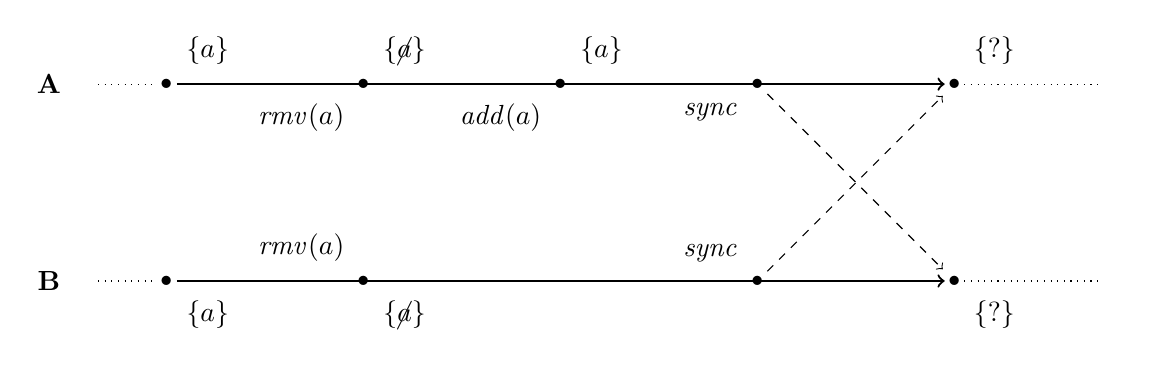
\begin{tikzpicture}
                \path
                    node {\textbf{A}}
                    ++(0:0.5) node (a) {}
                    +(0:13) node (a-end) {}
                    +(0:1) node[point, label=above right:{$\{a\}$}] (a-initial) {}
                    +(0:3.5) node (a-removes) {}
                    +(0:6) node (a-add) {}
                    +(0:8.5) node (a-start-sync) {}
                    +(0:11) node (a-end-sync) {};

                \path<2->
                    (a-removes) node[point, label=above right:{$\{\cancel{a}\}$}, label=below left:{$\trm{rmv}(a)$}] {}
                    (a-add) node[point, label=above right:{$\{a\}$}, label=below left:{$\trm{add}(a)$}] {};

                \draw[dotted] (a) -- (a-initial) (a-end-sync) -- (a-end);
                \draw[->, thick] (a-initial) -- (a-end-sync);

                \path
                    ++(270:2.5) node {\textbf{B}}
                    ++(0:0.5) node (b) {}
                    +(0:13) node (b-end) {}
                    +(0:1) node[point, label=below right:{$\{a\}$}] (b-initial) {}
                    +(0:3.5) node (b-removes) {}
                    +(0:8.5) node (b-start-sync) {}
                    +(0:11) node (b-end-sync) {};

                \path<3->
                    (b-removes) node[point, label=below right:{$\{\cancel{a}\}$}, label=above left:{$\trm{rmv}(a)$}] {};

                \path<4->
                    (a-start-sync) node[point, label=below left:{$\trm{sync}$}] {}
                    (a-end-sync) node[point, label=above right:{$\{?\}$}] {}
                    (b-start-sync) node[point, label=above left:{$\trm{sync}$}] {}
                    (b-end-sync) node[point, label=below right:{$\{?\}$}] {};

                \draw[dotted] (b) -- (b-initial) (b-end-sync) -- (b-end);
                \draw[->, thick] (b-initial) -- (b-end-sync);

                \draw<4->[->, dashed, shorten >= 1] (a-start-sync) edge (b-end-sync);
                \draw<4->[->, dashed, shorten >= 1] (b-start-sync) edge (a-end-sync);
            \end{tikzpicture}
        }
    \end{figure}
    \begin{itemize}
        \item<4-> \alert{What should be the final state} in this scenario ?
        \item<5-> Designing a CRDT consists in \alert{defining its behaviour} in such cases
    \end{itemize}
\end{frame}

\begin{frame}{Conflict Resolution Semantics - Case study of the Set}
    \metroset{block=transparent}
    \begin{figure}
        \resizebox{\textwidth}{!}{
            \centering
            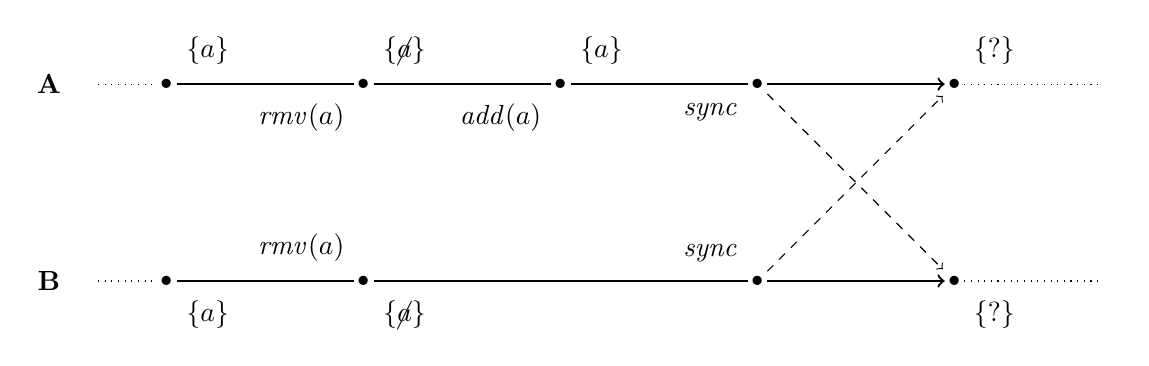
\begin{tikzpicture}
                \path
                    node {\textbf{A}}
                    ++(0:0.5) node (a) {}
                    +(0:13) node (a-end) {}
                    +(0:1) node[point, label=above right:{$\{a\}$}] (a-initial) {}
                    +(0:3.5) node[point, label=above right:{$\{\cancel{a}\}$}, label=below left:{$\trm{rmv}(a)$}] (a-removes) {}
                    +(0:6) node[point, label=above right:{$\{a\}$}, label=below left:{$\trm{add}(a)$}] (a-add) {}
                    +(0:8.5) node[point, label=below left:{$\trm{sync}$}] (a-start-sync) {}
                    +(0:11) node[point, label=above right:{$\{?\}$}] (a-end-sync) {};

                \draw[dotted] (a) -- (a-initial) (a-end-sync) -- (a-end);
                \draw[->, thick] (a-initial) --  (a-removes) -- (a-add) -- (a-start-sync) -- (a-end-sync);

                \path
                    ++(270:2.5) node {\textbf{B}}
                    ++(0:0.5) node (b) {}
                    +(0:13) node (b-end) {}
                    +(0:1) node[point, label=below right:{$\{a\}$}] (b-initial) {}
                    +(0:3.5) node[point, label=below right:{$\{\cancel{a}\}$}, label=above left:{$\trm{rmv}(a)$}] (b-removes) {}
                    +(0:8.5) node[point, label=above left:{$\trm{sync}$}] (b-start-sync) {}
                    +(0:11) node[point, label=below right:{$\{?\}$}] (b-end-sync) {};

                \draw[dotted] (b) -- (b-initial) (b-end-sync) -- (b-end);
                \draw[->, thick] (b-initial) --  (b-removes) -- (b-start-sync) -- (b-end-sync);

                \draw[->, dashed, shorten >= 1] (a-start-sync) edge (b-end-sync);
                \draw[->, dashed, shorten >= 1] (b-start-sync) edge (a-end-sync);
            \end{tikzpicture}
        }
    \end{figure}

    \begin{block}{Several semantics proposed:}
        \pause
        \begin{itemize}
            \item \emph{Add-Wins}: \alert{$\trm{add}(a)$ has priority} over concurrent $\trm{rmv}(a) \implies \{a\}$
            \pause
            \item \emph{Remove-Wins}: \alert{$\trm{rmv}(a)$ has priority} over concurrent $\trm{add}(a) \implies \{\cancel{a}\}$
            \pause
            \item \emph{Causal-Length} \cite{2020-cl-set-weihai}: The \alert{last action of the longuest chain of updates} determines the presence (or not) of the element $\implies \{a\}$
        \end{itemize}
    \end{block}
\end{frame}
\section{Synchronisation Models}

\begin{frame}{Synchronisation Models}
    \metroset{block=transparent}
    \begin{block}{To converge}
        \begin{itemize}
            \item Nodes have to propagate changes \dots
            \item \dots And integrate those of others
        \end{itemize}
    \end{block}

    \begin{block}{Several approaches proposed \cite{shapiro_2011_crdt}}
        \begin{itemize}
            \item State-based synchronisation
            \item Operation-based synchronisation
            \item<2->
                \only<2> {Delta-based synchronisation \cite{Almeida_2018}}
                \only<3> {\color{gray} Delta-based synchronisation \cite{Almeida_2018}}
            \only<2-3>{
                \begin{itemize}
                    \item
                        \only<2>{"Best of the two worlds" approach}
                        \only<3>{\color{gray} "Best of the two worlds" approach}
                \end{itemize}
            }
        \end{itemize}
    \end{block}
\end{frame}


\begin{frame}{An aparté about lattice theory}
    \metroset{block=transparent}

    \begin{block}{Properties of join-semilattices}
        \begin{itemize}
            \item States of the join-semilattices are partially ordered according to relation $\leq$
            \item Updates produce new states by inflation, i.e. greater to previous ones according to $\leq$
            \item Exists a function $\trm{join}$ that, given any pair of states, generates the minimal state greater or equal to both given states according to $\leq$
            \item Exists a set of minimal states of the join-semilattice, the \emph{irreducible elements}
        \end{itemize}
    \end{block}
\end{frame}

\subsection{State-based CRDTs}

\begin{frame}{State-based synchronisation}
    \metroset{block=transparent}

    \begin{itemize}
        \item \alert{Send periodically current state} to other nodes
    \end{itemize}

    \begin{figure}[!ht]

        \centering
        \resizebox{\columnwidth}{!}{
          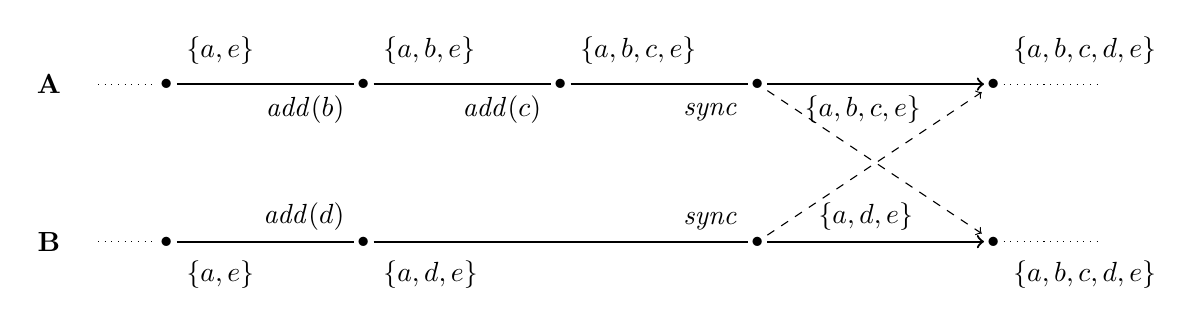
\begin{tikzpicture}
            \path
                node {\textbf{A}}
                ++(0:0.5) node (a) {}
                +(0:13) node (a-end) {}
                +(0:1) node[point, label=above right:{$\set{a,e}$}] (a-initial) {}
                +(0:3.5) node[point, label=above right:{$\set{a,b,e}$}, label=-170:{$\trm{add}(b)$}] (a-add-b) {}
                +(0:6) node[point, label=above right:{$\set{a,b,c,e}$}, label=-170:{$\trm{add}(c)$}] (a-add-c) {}
                +(0:8.5) node[point, label=below left:{$\trm{sync}$}, label={[xshift=10pt]-10:{$\set{a,b,c,e}$}}] (a-sends-state) {}
                +(0:11.5) node[point, label=above right:{$\set{a,b,c,d,e}$}] (a-final) {};

            \draw[dotted] (a) -- (a-initial) (a-final) -- (a-end);
            \draw[->, thick] (a-initial) --  (a-add-b) -- (a-add-c) -- (a-sends-state) -- (a-final);

            \path
                ++(270:2) node {\textbf{B}}
                ++(0:0.5) node (b) {}
                +(0:13) node (b-end) {}
                +(0:1) node[point, label=below right:{$\set{a,e}$}] (b-initial) {}
                +(0:3.5) node[point, label=below right:{$\set{a,d,e}$}, label=170:{$\trm{add}(d)$}] (b-add-d) {}
                +(0:8.5) node[point, label=170:{$\trm{sync}$}, label={[xshift=15pt]10:{$\set{a,d,e}$}}] (b-sends-state) {}
                +(0:11.5) node[point, label=below right:{$\set{a,b,c,d,e}$}] (b-final) {};

            \draw[dotted] (b) -- (b-initial) (b-final) -- (b-end);
            \draw[->, thick] (b-initial) --  (b-add-d) -- (b-sends-state) -- (b-final);

            \draw[->, dashed, shorten >= 1] (a-sends-state) -- (b-final);
            \draw[->, dashed, shorten >= 1] (b-sends-state) -- (a-final);
          \end{tikzpicture}
        }
    \end{figure}

    \begin{itemize}
        \item Upon reception, \alert{computes new state by merging received state with current one} using \texttt{merge} function
        \item With \texttt{merge}, a \alert{commutative, associative and idempotent function}
    \end{itemize}
\end{frame}

\begin{frame}{State-based synchronisation - ???}
    \metroset{block=transparent}

    \begin{block}{Strengths}
        \begin{itemize}
            \item No assumptions on the network reliability
            \item i.e. messages may be lost, re-ordered or duplicated w/o impact
        \end{itemize}
    \end{block}
    \begin{block}{Limits}
        \begin{itemize}
            \item States difficult to design
            \begin{itemize}
                \item e.g. how to represent efficiently deletion of elements?
            \end{itemize}
            \item States expensive to broadcast
            \item \texttt{merge} expensive
        \end{itemize}
    \end{block}
\end{frame}

\subsection{Operation-based CRDTs}

\begin{frame}{Operation-based synchronisation}
    \begin{itemize}
        \item \alert{Encode updates as arbitrary messages}, called \emph{operations}
        \item An operation \alert{correponds to one or several irreducible elements}
    \end{itemize}

    \begin{figure}[!ht]

        \centering
        \resizebox{\columnwidth}{!}{
          \begin{tikzpicture}
            \path
                node {\textbf{A}}
                ++(0:0.5) node (a) {}
                +(0:17) node (a-end) {}
                +(0:1) node[point, label=above right:{$\set{a,e}$}] (a-initial) {}
                +(0:3.5) node[point, label=above right:{$\set{a,b,e}$}, label=-170:{$\trm{add}(b)$}] (a-add-b) {}
                +(0:6) node[point, label=above right:{$\set{a,b,c,e}$}, label=-170:{$\trm{add}(c)$}] (a-add-c) {}
                +(0:8.5) node[point, label=above right:{$\set{a,b,c,d,e}$}] (a-receives-add-d) {}
                +(0:13.5) node[point, label={[xshift=8pt]-10:{$\trm{add(b)}$}}] (a-receives-query-sync) {}
                +(0:16) node (a-final) {};

            \draw[dotted] (a) -- (a-initial) (a-final) -- (a-end);
            \draw[->, thick] (a-initial) --  (a-add-b) -- (a-add-c) -- (a-receives-add-d) -- (a-receives-query-sync) -- (a-final);

            \path
                ++(270:3) node {\textbf{B}}
                ++(0:0.5) node (b) {}
                +(0:17) node (b-end) {}
                +(0:1) node[point, label=below right:{$\set{a,e}$}] (b-initial) {}
                +(0:6) node[point, label=below right:{$\set{a,d,e}$}, label=170:{$\trm{add}(d)$}] (b-add-d) {}
                +(0:8.5) node[point, label=below right:{$\set{a,c,d,e}$}] (b-receives-add-c) {}
                +(0:11) node[point, label=170:{$\trm{query\ sync}$}] (b-sends-query-sync) {}
                +(0:16) node[point, label=below right:{$\set{a,b,c,d,e}$}] (b-final) {};

            \draw[dotted] (b) -- (b-initial) (b-final) -- (b-end);
            \draw[->, thick] (b-initial) --  (b-add-d) -- (b-receives-add-c) -- (b-sends-query-sync) -- (b-final);

            \draw[->, dashed, shorten >= 1] (a-add-c) -- (b-receives-add-c);
            \draw[->, dashed, shorten >= 1] (b-add-d) -- (a-receives-add-d);
            \draw[->, dashed, shorten >= 1] (b-sends-query-sync) -- (a-receives-query-sync);
            \draw[->, dashed, shorten >= 1] (a-receives-query-sync) -- (b-final);

            \path
              ++(270:1.5)
              ++(0:0.5)
              +(0:4.75) node[cross] (network-error) {};

            \draw[->, dashed, shorten >= 1] (a-add-b) -- (network-error);
          \end{tikzpicture}
        }
      \end{figure}

    \begin{itemize}
        \item Upon reception, \alert{apply operations on current state}
        \item \alert{Concurrent operations} must be \alert{commutative}
    \end{itemize}
\end{frame}

\begin{frame}{Operation-based synchronisation - ???}
    \metroset{block=transparent}

    \begin{block}{Strengths}
        \begin{itemize}
            \item Designing operations is straightforward
            \item Operations usually cheap to broadcast and apply
        \end{itemize}
    \end{block}
    \begin{block}{Limits}
        \begin{itemize}
            \item Hides/delegates complexity to delivery of operations
            \begin{itemize}
                \item i.e. requires specific delivery order of operations
                \item e.g. insertion of an element before its deletion
            \end{itemize}
            \item Have to pair Op-based CRDTs with a delivery service to handle network failures
            \begin{itemize}
                \item To re-order and/or de-duplicate operations
                \item To retrieve lost operations using anti-entropy mechanisms
            \end{itemize}
        \end{itemize}
    \end{block}
\end{frame}
\input{content/state-of-art}

\begin{frame}[allowframebreaks]{Bibliographie}
    \vspace{1em}
    \printbibliography%
\end{frame}


\begin{frame}[standout]
    \alert{Back-up slides}
\end{frame}

\section{Synchronisation Models}

\subsection{Operation-based synchronisation}

\begin{frame}{Operation-based synchronisation - network failure}
    \begin{figure}[!ht]

        \centering
        \resizebox{\columnwidth}{!}{
          \begin{tikzpicture}
            \path
                node {\textbf{A}}
                ++(0:0.5) node (a) {}
                +(0:17) node (a-end) {}
                +(0:1) node[point, label=above right:{$\set{a,e}$}] (a-initial) {}
                +(0:3.5) node[point, label=above right:{$\set{a,b,e}$}, label=-170:{$\trm{add}(b)$}] (a-add-b) {}
                +(0:6) node[point, label=above right:{$\set{a,b,c,e}$}, label=-170:{$\trm{add}(c)$}] (a-add-c) {}
                +(0:8.5) node[point, label=above right:{$\set{a,b,c,d,e}$}] (a-receives-add-d) {}
                +(0:13.5) node[point, label={[xshift=8pt]-10:{$\trm{add(b)}$}}] (a-receives-query-sync) {}
                +(0:16) node (a-final) {};

            \draw[dotted] (a) -- (a-initial) (a-final) -- (a-end);
            \draw[->, thick] (a-initial) --  (a-add-b) -- (a-add-c) -- (a-receives-add-d) -- (a-receives-query-sync) -- (a-final);

            \path
                ++(270:3) node {\textbf{B}}
                ++(0:0.5) node (b) {}
                +(0:17) node (b-end) {}
                +(0:1) node[point, label=below right:{$\set{a,e}$}] (b-initial) {}
                +(0:6) node[point, label=below right:{$\set{a,d,e}$}, label=170:{$\trm{add}(d)$}] (b-add-d) {}
                +(0:8.5) node[point, label=below right:{$\set{a,c,d,e}$}] (b-receives-add-c) {}
                +(0:11) node[point, label=170:{$\trm{query\ sync}$}] (b-sends-query-sync) {}
                +(0:16) node[point, label=below right:{$\set{a,b,c,d,e}$}] (b-final) {};

            \draw[dotted] (b) -- (b-initial) (b-final) -- (b-end);
            \draw[->, thick] (b-initial) --  (b-add-d) -- (b-receives-add-c) -- (b-sends-query-sync) -- (b-final);

            \draw[->, dashed, shorten >= 1] (a-add-c) -- (b-receives-add-c);
            \draw[->, dashed, shorten >= 1] (b-add-d) -- (a-receives-add-d);
            \draw[->, dashed, shorten >= 1] (b-sends-query-sync) -- (a-receives-query-sync);
            \draw[->, dashed, shorten >= 1] (a-receives-query-sync) -- (b-final);

            \path
              ++(270:1.5)
              ++(0:0.5)
              +(0:4.75) node[cross] (network-error) {};

            \draw[->, dashed, shorten >= 1] (a-add-b) -- (network-error);
          \end{tikzpicture}
        }
    \end{figure}
\end{frame}

\subsection{Delta-based synchronisation}

\subsection{Recap}

\begin{frame}{Synchronisation Models - Summary}
    \begin{table}[!ht]
        \centering
        \resizebox{\columnwidth}{!}{
          \begin{tabular}{lccc}
            \toprule
                                                      & State-based & Op-based    & Delta-based \\
            \midrule
            Integrate updates by merging states         & \checkmark  & \ballotx    & \checkmark  \\
            Integrate updates by irreducible elts      & \ballotx    & \checkmark  & \checkmark  \\
            Handle natively network failures          & \checkmark  & \ballotx    & \checkmark  \\
            Suited for real-time systems              & \ballotx    & \checkmark  & \checkmark  \\
            \bottomrule
          \end{tabular}
        }
    \end{table}
\end{frame}
\section{MUTE}

\begin{frame}{Architecture système de MUTE}
    \vspace{-0.5cm}
    \begin{figure}
        \resizebox{\textwidth}{!}{
            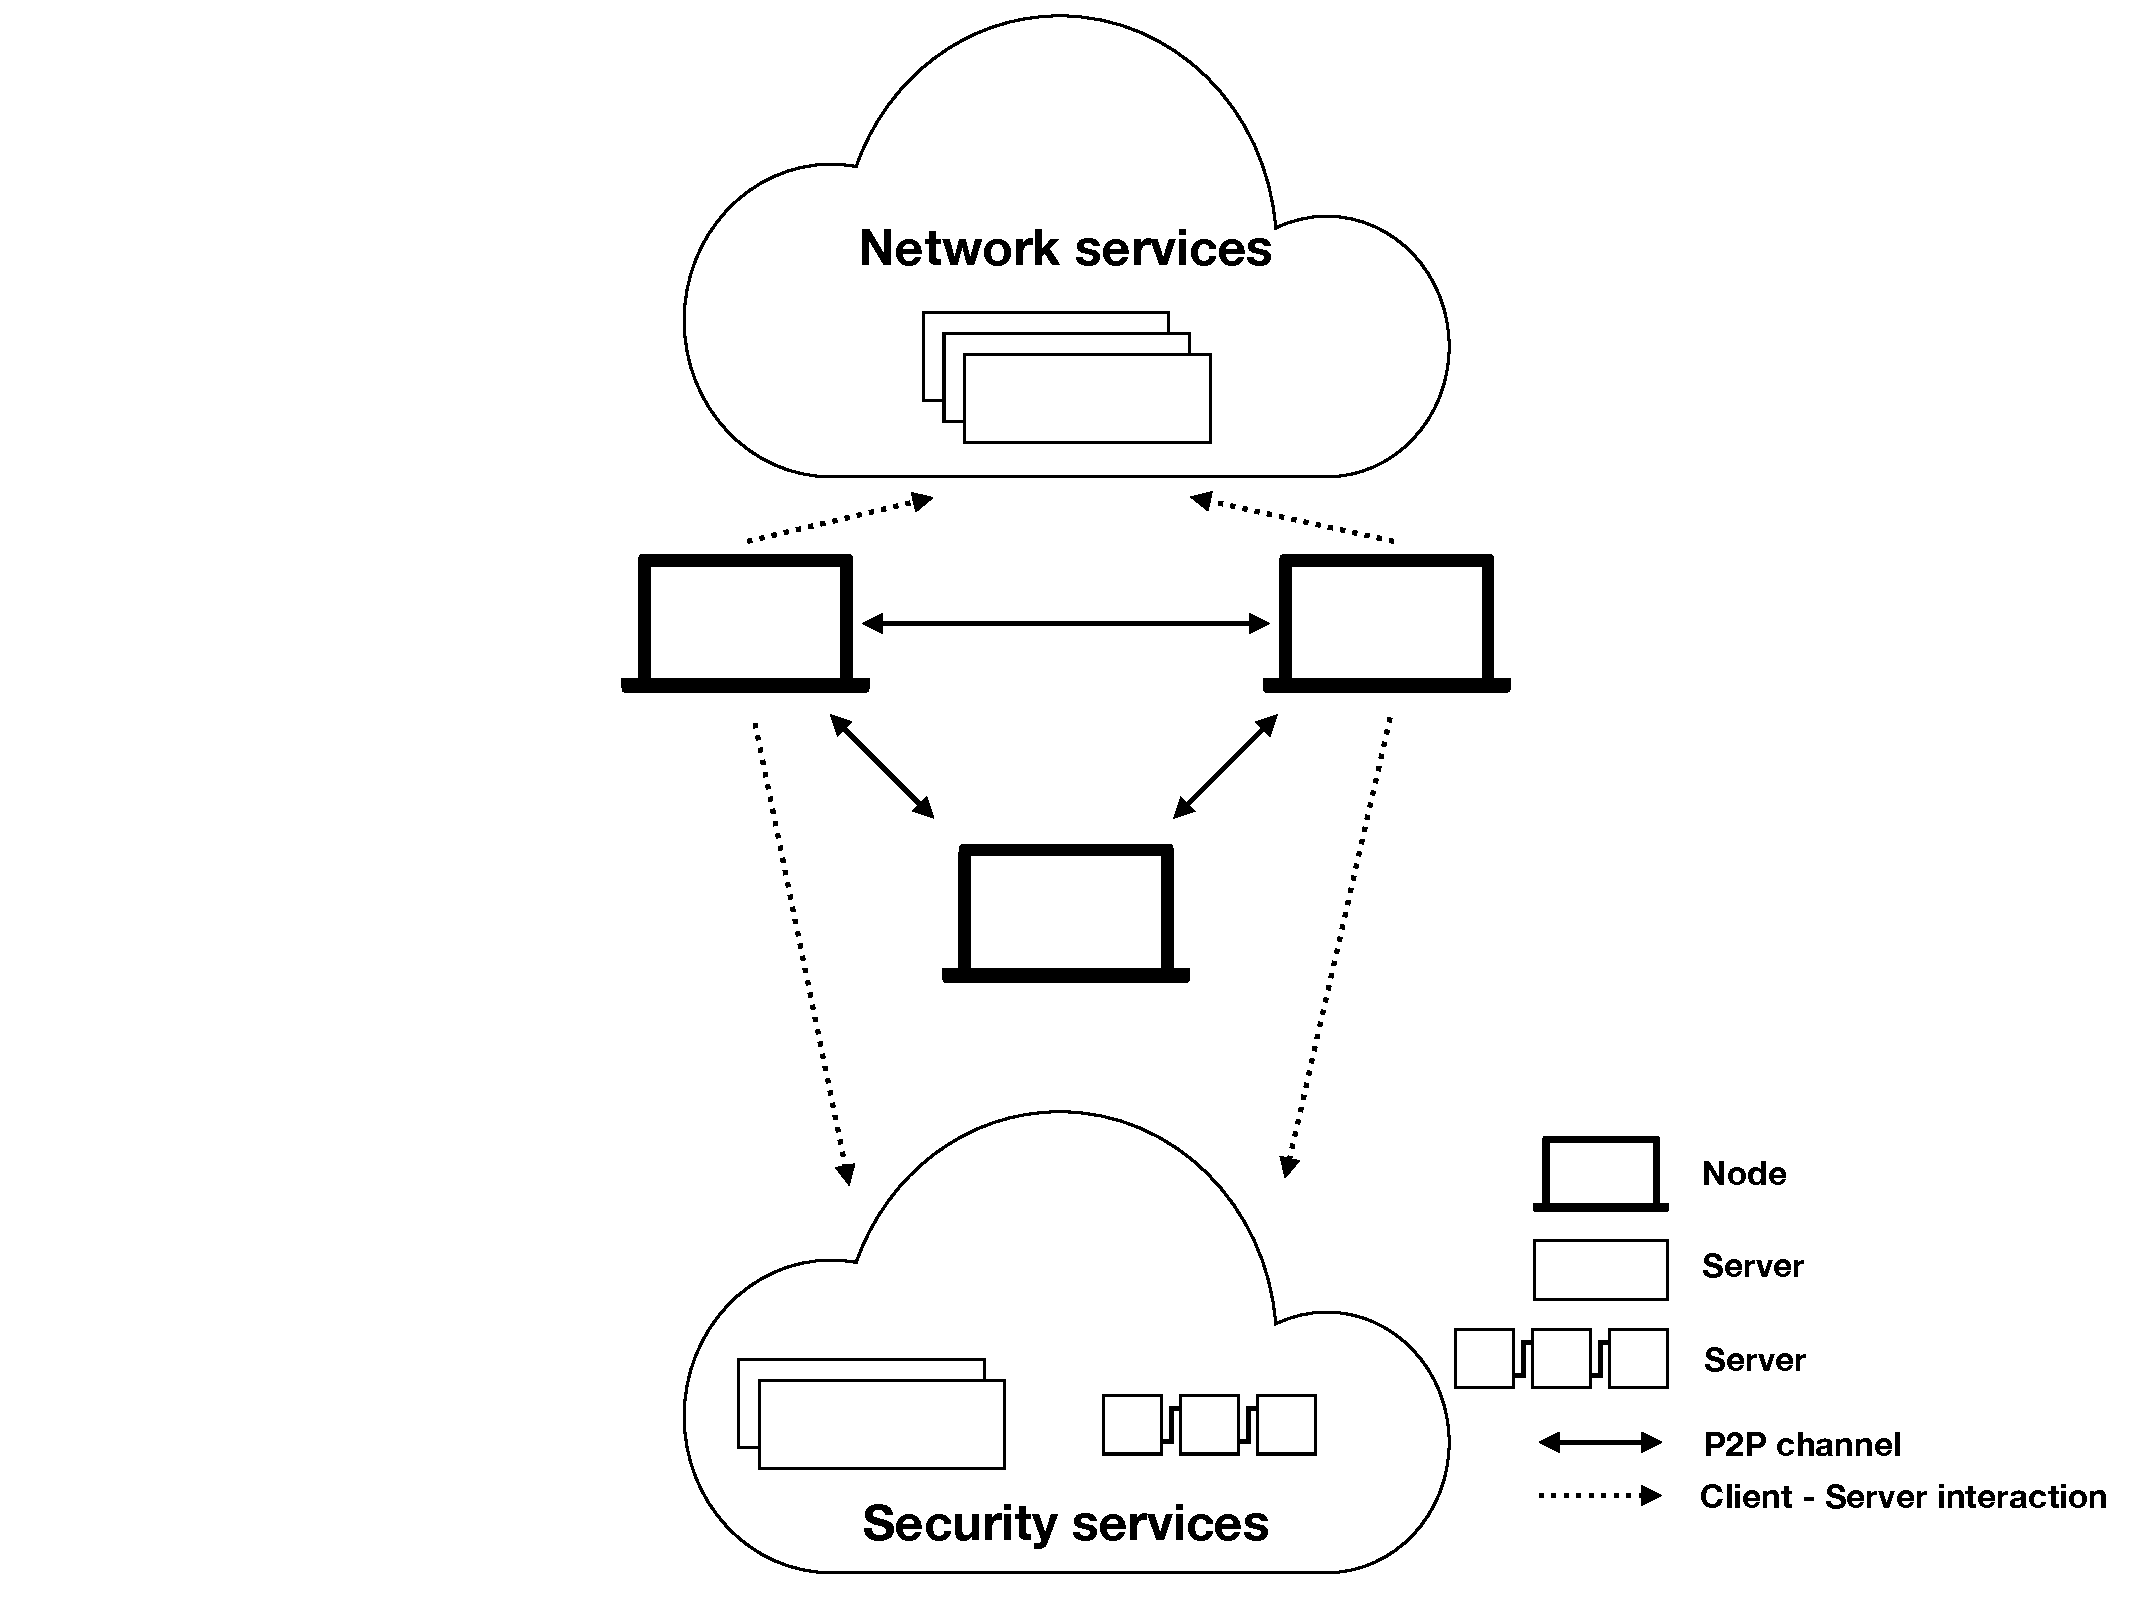
\includegraphics[page=1, trim=0cm 0cm 0cm 0cm, clip, width=.7\linewidth]{img/mute-figures.pdf}
            }
    \end{figure}
\end{frame}


\begin{frame}{Architecture logicielle de MUTE}
    \vspace{-0.5cm}
    \begin{figure}
        \resizebox{\textwidth}{!}{
            \includegraphics[page=2, trim=0cm 0cm 0cm 0cm, clip, width=.7\linewidth]{img/mute-figures.pdf}
        }
    \end{figure}
\end{frame}

\begin{frame}{Contributions}
    \metroset{block=transparent}
    \begin{block}{Document}
        \begin{itemize}
            \item Implémentation des CRDTs LogootSplit et RenamableLogootSplit
        \end{itemize}
    \end{block}

    \begin{block}{Operation Dependancies \& Anti-Entropy}
        \begin{itemize}
            \item Implémentation des modèles de livraison pour LogootSplit et RenamableLogootSplit
            \item Implémentation d'un mécanisme d'anti-entropie (détection et échange des opérations perdues)
        \end{itemize}
    \end{block}

    \begin{block}{Ingénierie logicielle}
        \begin{itemize}
            \item Mise en place des processus d'intégration continue et de livraison continue pour les librairies \texttt{mute-structs}\singlefootnote{\url{https://github.com/coast-team/mute-structs}} et \texttt{mute-core}\singlefootnote{\url{https://github.com/coast-team/mute-core}}
        \end{itemize}
    \end{block}
\end{frame}

\begin{frame}{Contributions - suite}
    \metroset{block=transparent}
    \begin{block}{Network}
        \begin{itemize}
            \item Supervision de la réalisation d'un \emph{Proof of Concept} basé sur l'utilisation d'un \emph{log-based message broker}
        \end{itemize}
    \end{block}

    \begin{block}{Collaborators}
        \begin{itemize}
            \item Supervision de l'adaptation et l'implémentation de SWIM, un protocole d'appartenance au réseau
        \end{itemize}
    \end{block}
\end{frame}


\end{document}
